% \documentclass[onecolumn]{article}
\documentclass[twocolumn]{article}

\usepackage{style/arxiv}

% --- Packages ---
\usepackage[utf8]{inputenc}
\usepackage[T1]{fontenc}
\usepackage{amsmath, amssymb, amsthm}
\usepackage{hyperref}
\usepackage{cleveref}
\usepackage{url}
\usepackage{booktabs}
\usepackage{amsfonts}
\usepackage{nicefrac}
\usepackage{microtype}
\usepackage{xcolor}
\usepackage{graphicx}
\usepackage{subcaption}
\usepackage{wrapfig}
\usepackage{enumitem}
\usepackage[ruled,vlined]{algorithm2e}

\graphicspath{{figures/}}

% Shared macros for the paper.

\newcommand{\method}{MethodName}


\crefname{algocf}{algorithm}{algorithms}
\Crefname{algocf}{Algorithm}{Algorithms}

% --- Theorem-like environments ---
\newtheorem{theorem}{Theorem}[section]
\newtheorem{lemma}[theorem]{Lemma}
\newtheorem{corollary}[theorem]{Corollary}
\newtheorem{proposition}[theorem]{Proposition}

\theoremstyle{definition}
\newtheorem{definition}[theorem]{Definition}
\newtheorem{condition}[theorem]{Condition}
\newtheorem{example}[theorem]{Example}

\theoremstyle{remark}
\newtheorem*{remark}{Remark}
\newtheorem*{note}{Note}

% --- Paper metadata ---
\title{Paper Title}

\author{%
  Author Name \\
  Affiliation \\
  \texttt{email@example.com}
}

\hypersetup{
  pdftitle={Paper Title},
  pdfauthor={Author Name},
  pdfkeywords={Keyword 1, Keyword 2}
}

\begin{document}

\maketitle

\begin{abstract}
Write the paper abstract here.

\end{abstract}

\section{Introduction}
\label{sec:introduction}

Write the introduction here.

\section{Related Work}
\label{sec:related-work}

Write the related work here.

\section{Method}
\label{sec:method}

Write the method here.

\section{Experiments}
\label{sec:experiments}

Write the experiments here.

% Example float snippets:
% \begin{figure}[t]
  \centering
  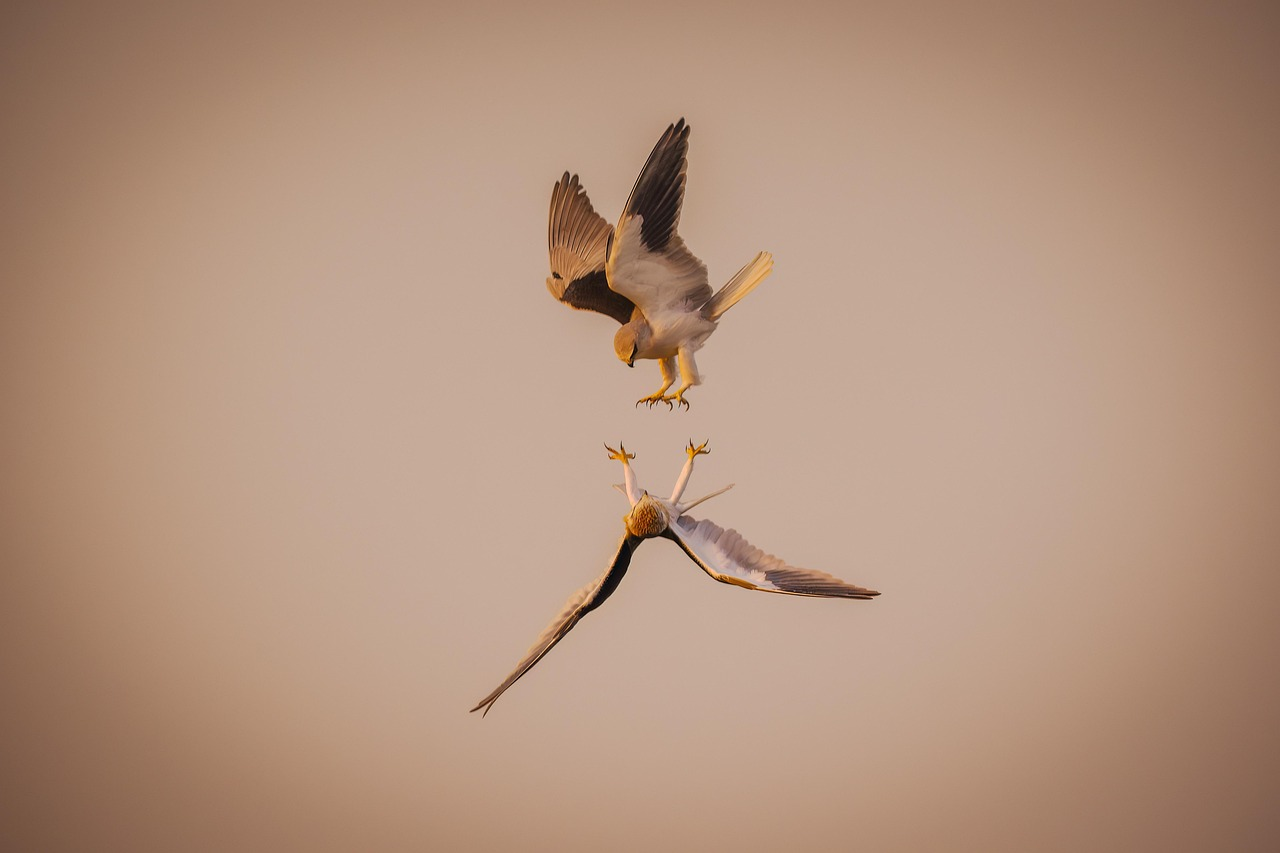
\includegraphics[width=\linewidth]{example1.jpg}
  \caption{Main figure caption.}
  \label{fig:main}
\end{figure}

% \begin{table}[t]
  \caption{Main results.}
  \label{tab:main-results}
  \centering
  \begin{tabular}{lcc}
    \toprule
    Method & Metric 1 & Metric 2 \\
    \midrule
    Baseline & -- & -- \\
    \method{} & -- & -- \\
    \bottomrule
  \end{tabular}
\end{table}


\section{Conclusion}
\label{sec:conclusion}

Write the conclusion here.

\section{Limitations}
\label{sec:limitations}

Write the limitations here.


% \section*{Acknowledgments}
% \input{sections/acknowledgments}

\bibliographystyle{unsrtnat}
\bibliography{references}

\appendix
\onecolumn
\section{Appendix}
\label{sec:appendix}

Write appendix material here.


\end{document}
